\documentclass[11pt]{beamer}
\usepackage{lmodern}
\usepackage{graphicx}
\usepackage{hyperref}
\usetheme{Singapore}
\author{Gerd Graßhoff}
\title{Algorithmische Geschichte und Philosophie der Wissenschaften, Vorl 3}
\date{2. Mai 2019}

\begin{document}
	\begin{frame}[plain]
		\maketitle
	\end{frame}
	

\section{Exoplanet}

\begin{frame}
	\frametitle{Bisherige Entdeckungen}
	\centering
	\href{https://exoplanets.nasa.gov/}{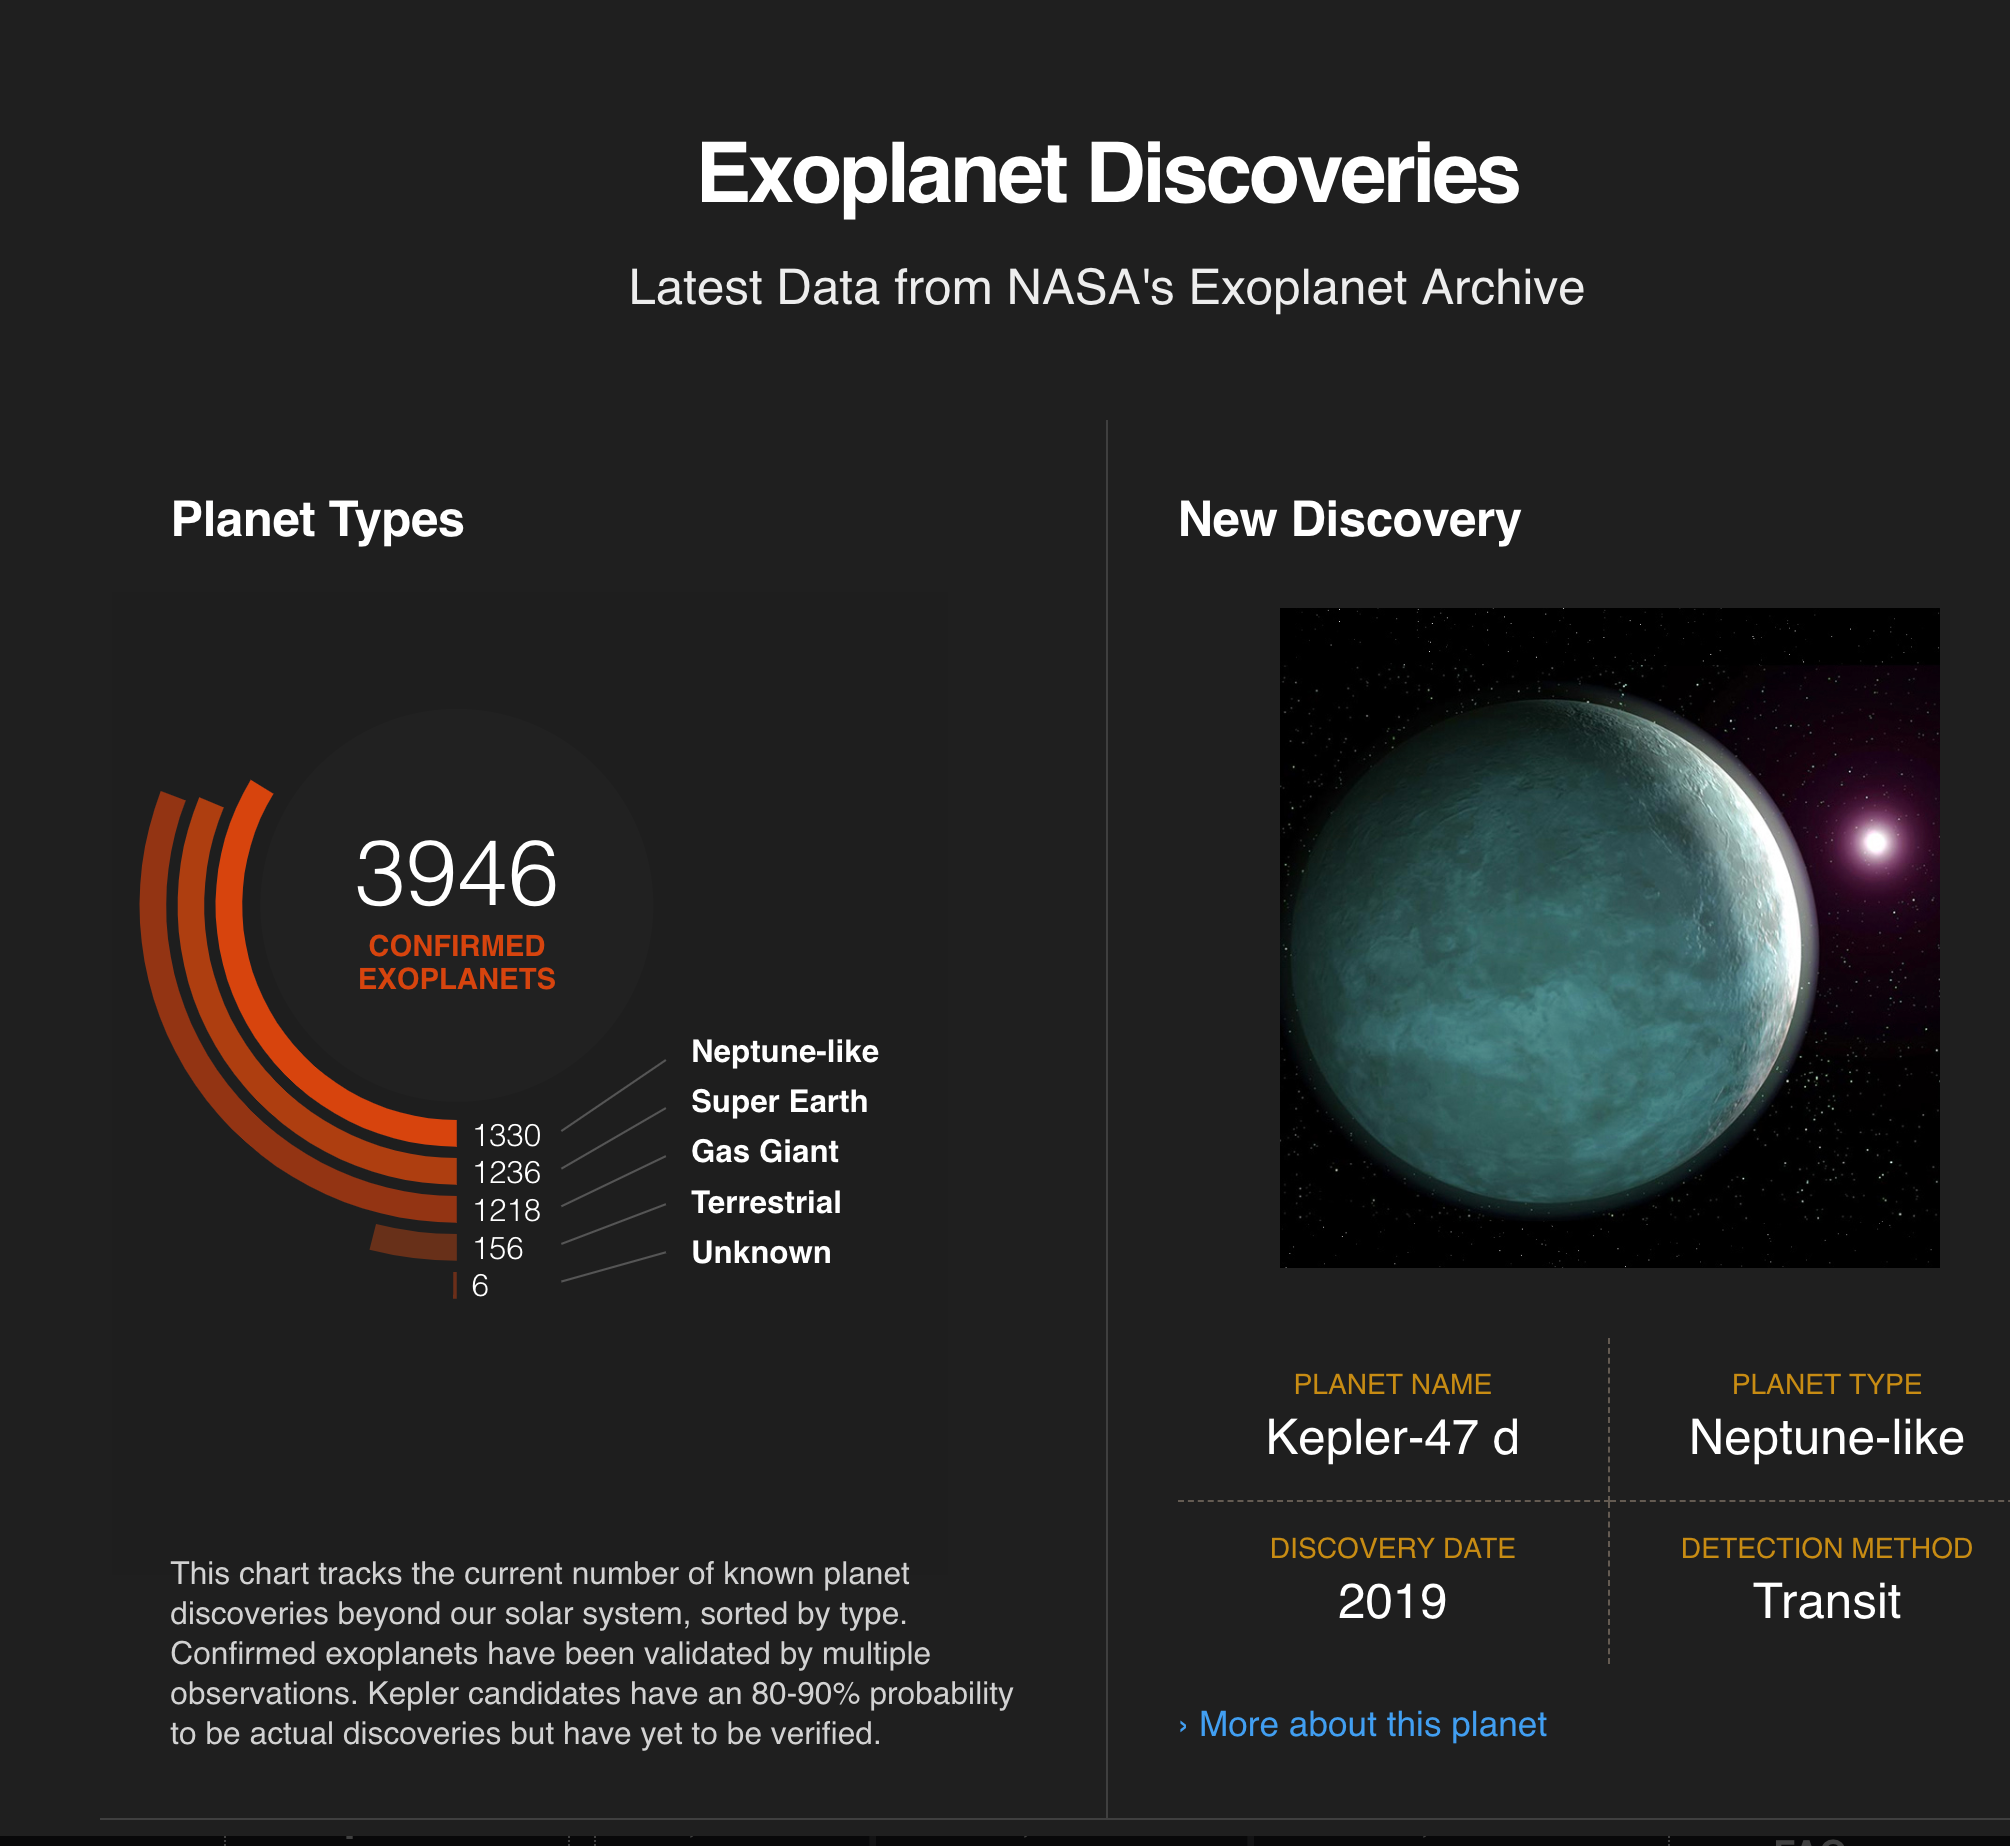
\includegraphics[width=1\linewidth]{screenshot001}}
	
\end{frame}

\begin{frame}
	\frametitle{Forschungsgeschichte}
	\centering
	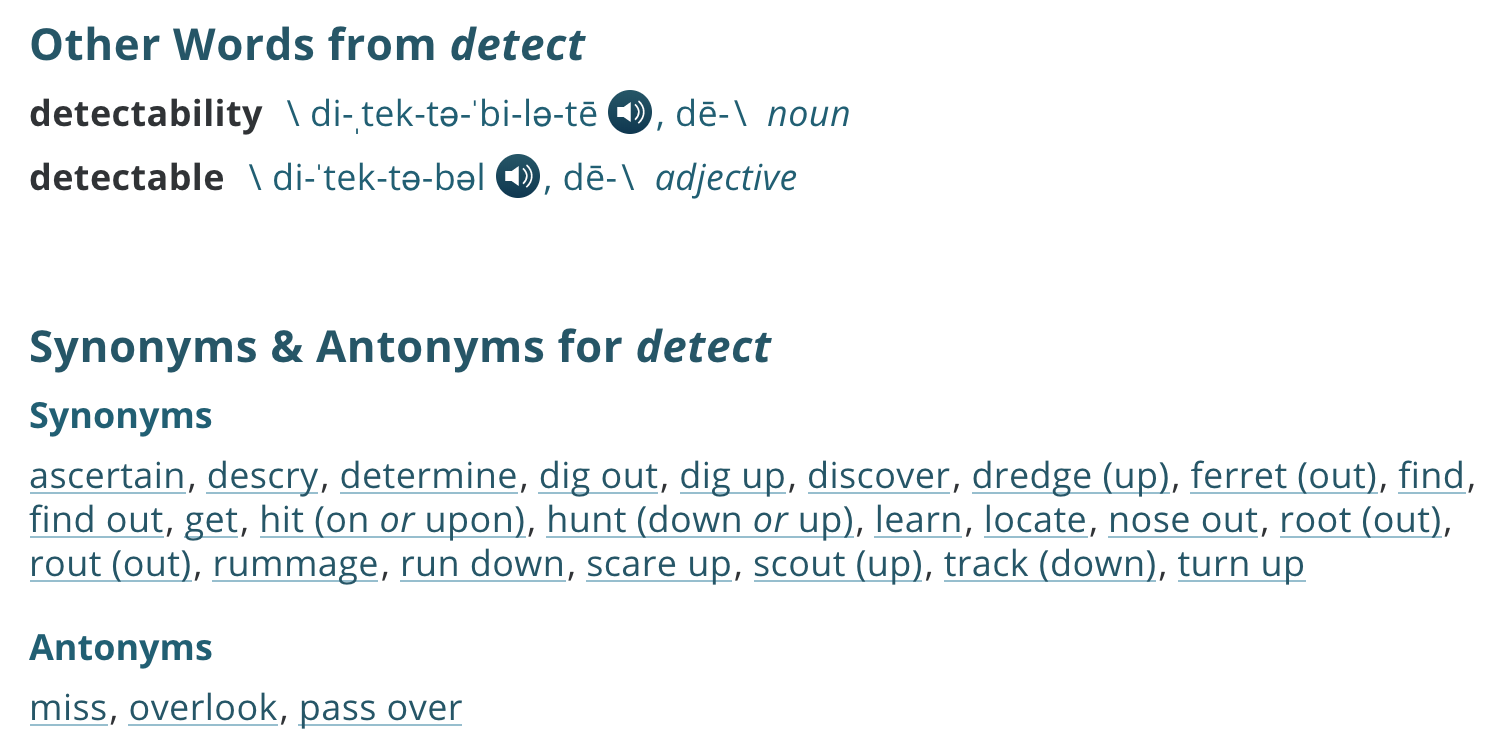
\includegraphics[width=1\linewidth]{screenshot002}
\end{frame}


\begin{frame}
	\frametitle{Messungen}
	
	\begin{itemize}
		\item\href{https://exoplanets.nasa.gov/5-ways-to-find-a-planet/}{Messungen}
		\item\href{https://exoplanetarchive.ipac.caltech.edu/cgi-bin/TblView/nph-tblView?app=ExoTbls&config=planets}{Planetentabelle}
		\item\href{https://www.nasa.gov/mission_pages/kepler/overview/index.html}{Kepler Mission}
	\end{itemize}
\end{frame}

	\begin{frame}
	\frametitle{Wissenschaftstheoretische Schlüsselbegriffe}
	\begin{itemize}
		\item Forschungsobjekt / System / Planetensystem
		\item Modell
		\item Messung / Data
		\begin{itemize}
			\item Messverfahren / -prozess
			\item Instrument
		\end{itemize}
		\item Befund / Ergebnis / Entdeckung
		\item Forschungsbewertung / -Vergleich
	\end{itemize}
\end{frame}


\begin{frame}
	\frametitle{Arten der Entdeckung}
	\begin{figure}
		\centering
		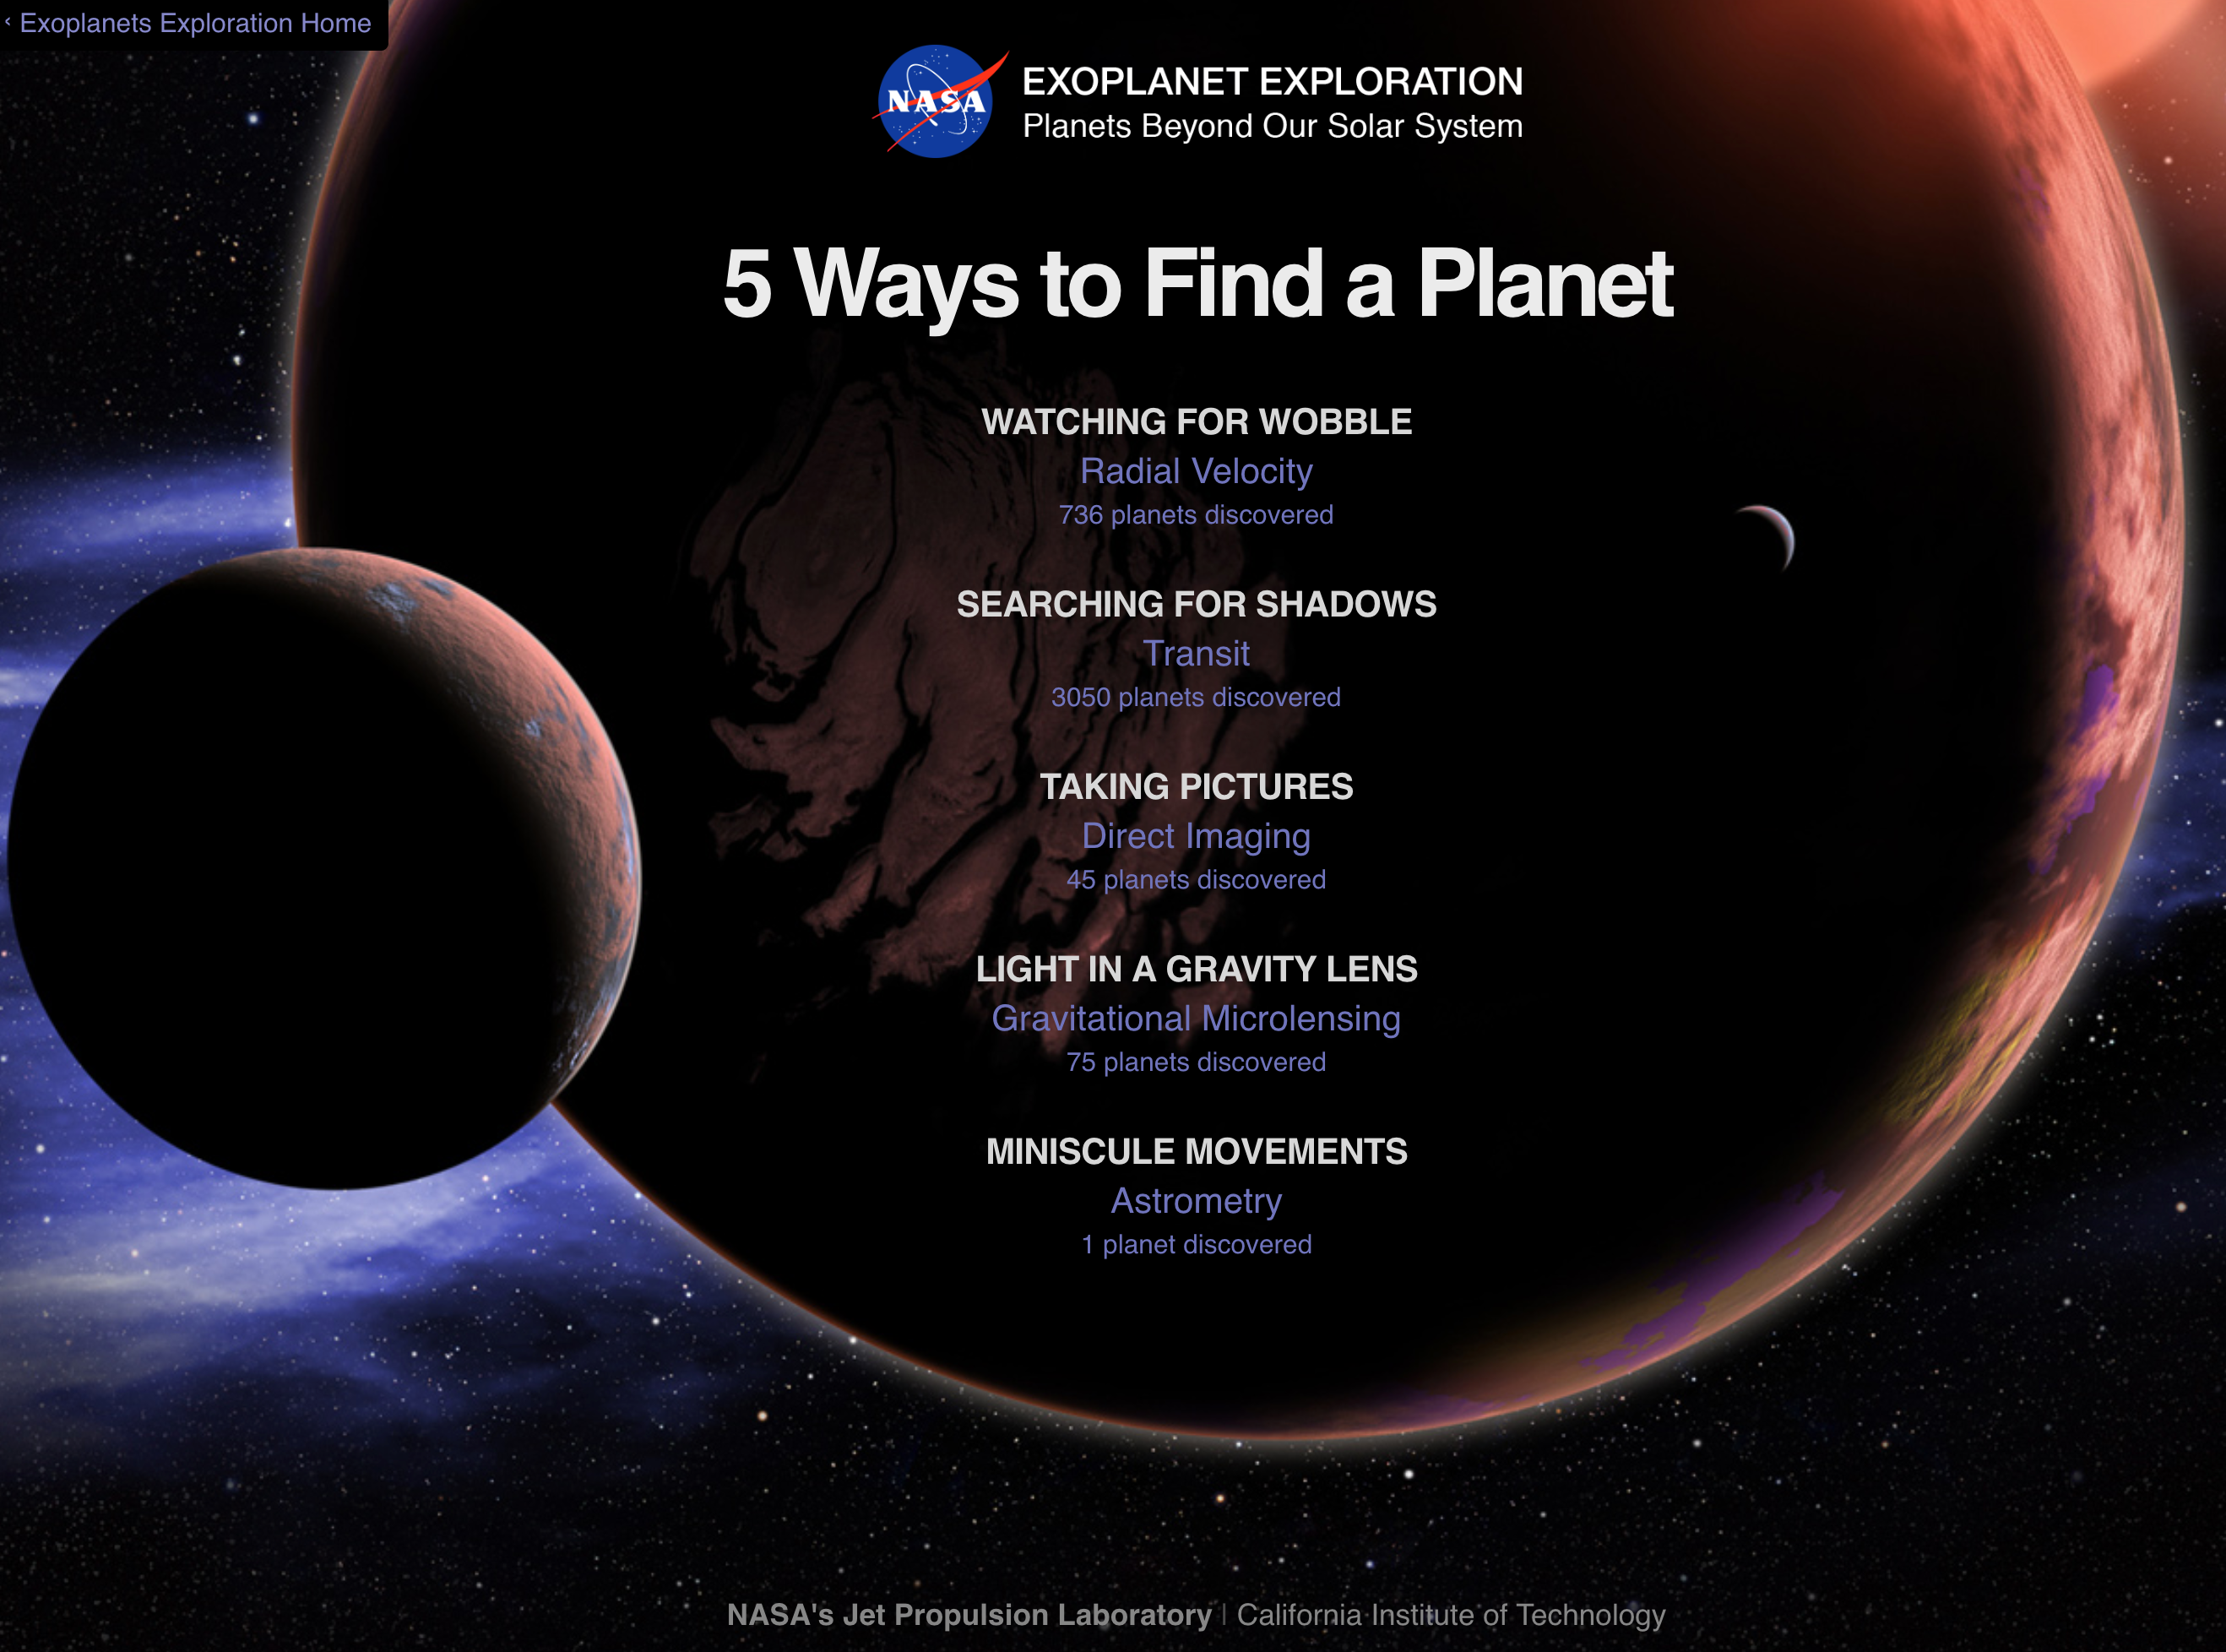
\includegraphics[width=1\linewidth]{screenshot004}
		\caption{}
		\label{fig:screenshot004}
	\end{figure}
	
\end{frame}

\begin{frame}
	\frametitle{NASA Archiv}
	\centering
	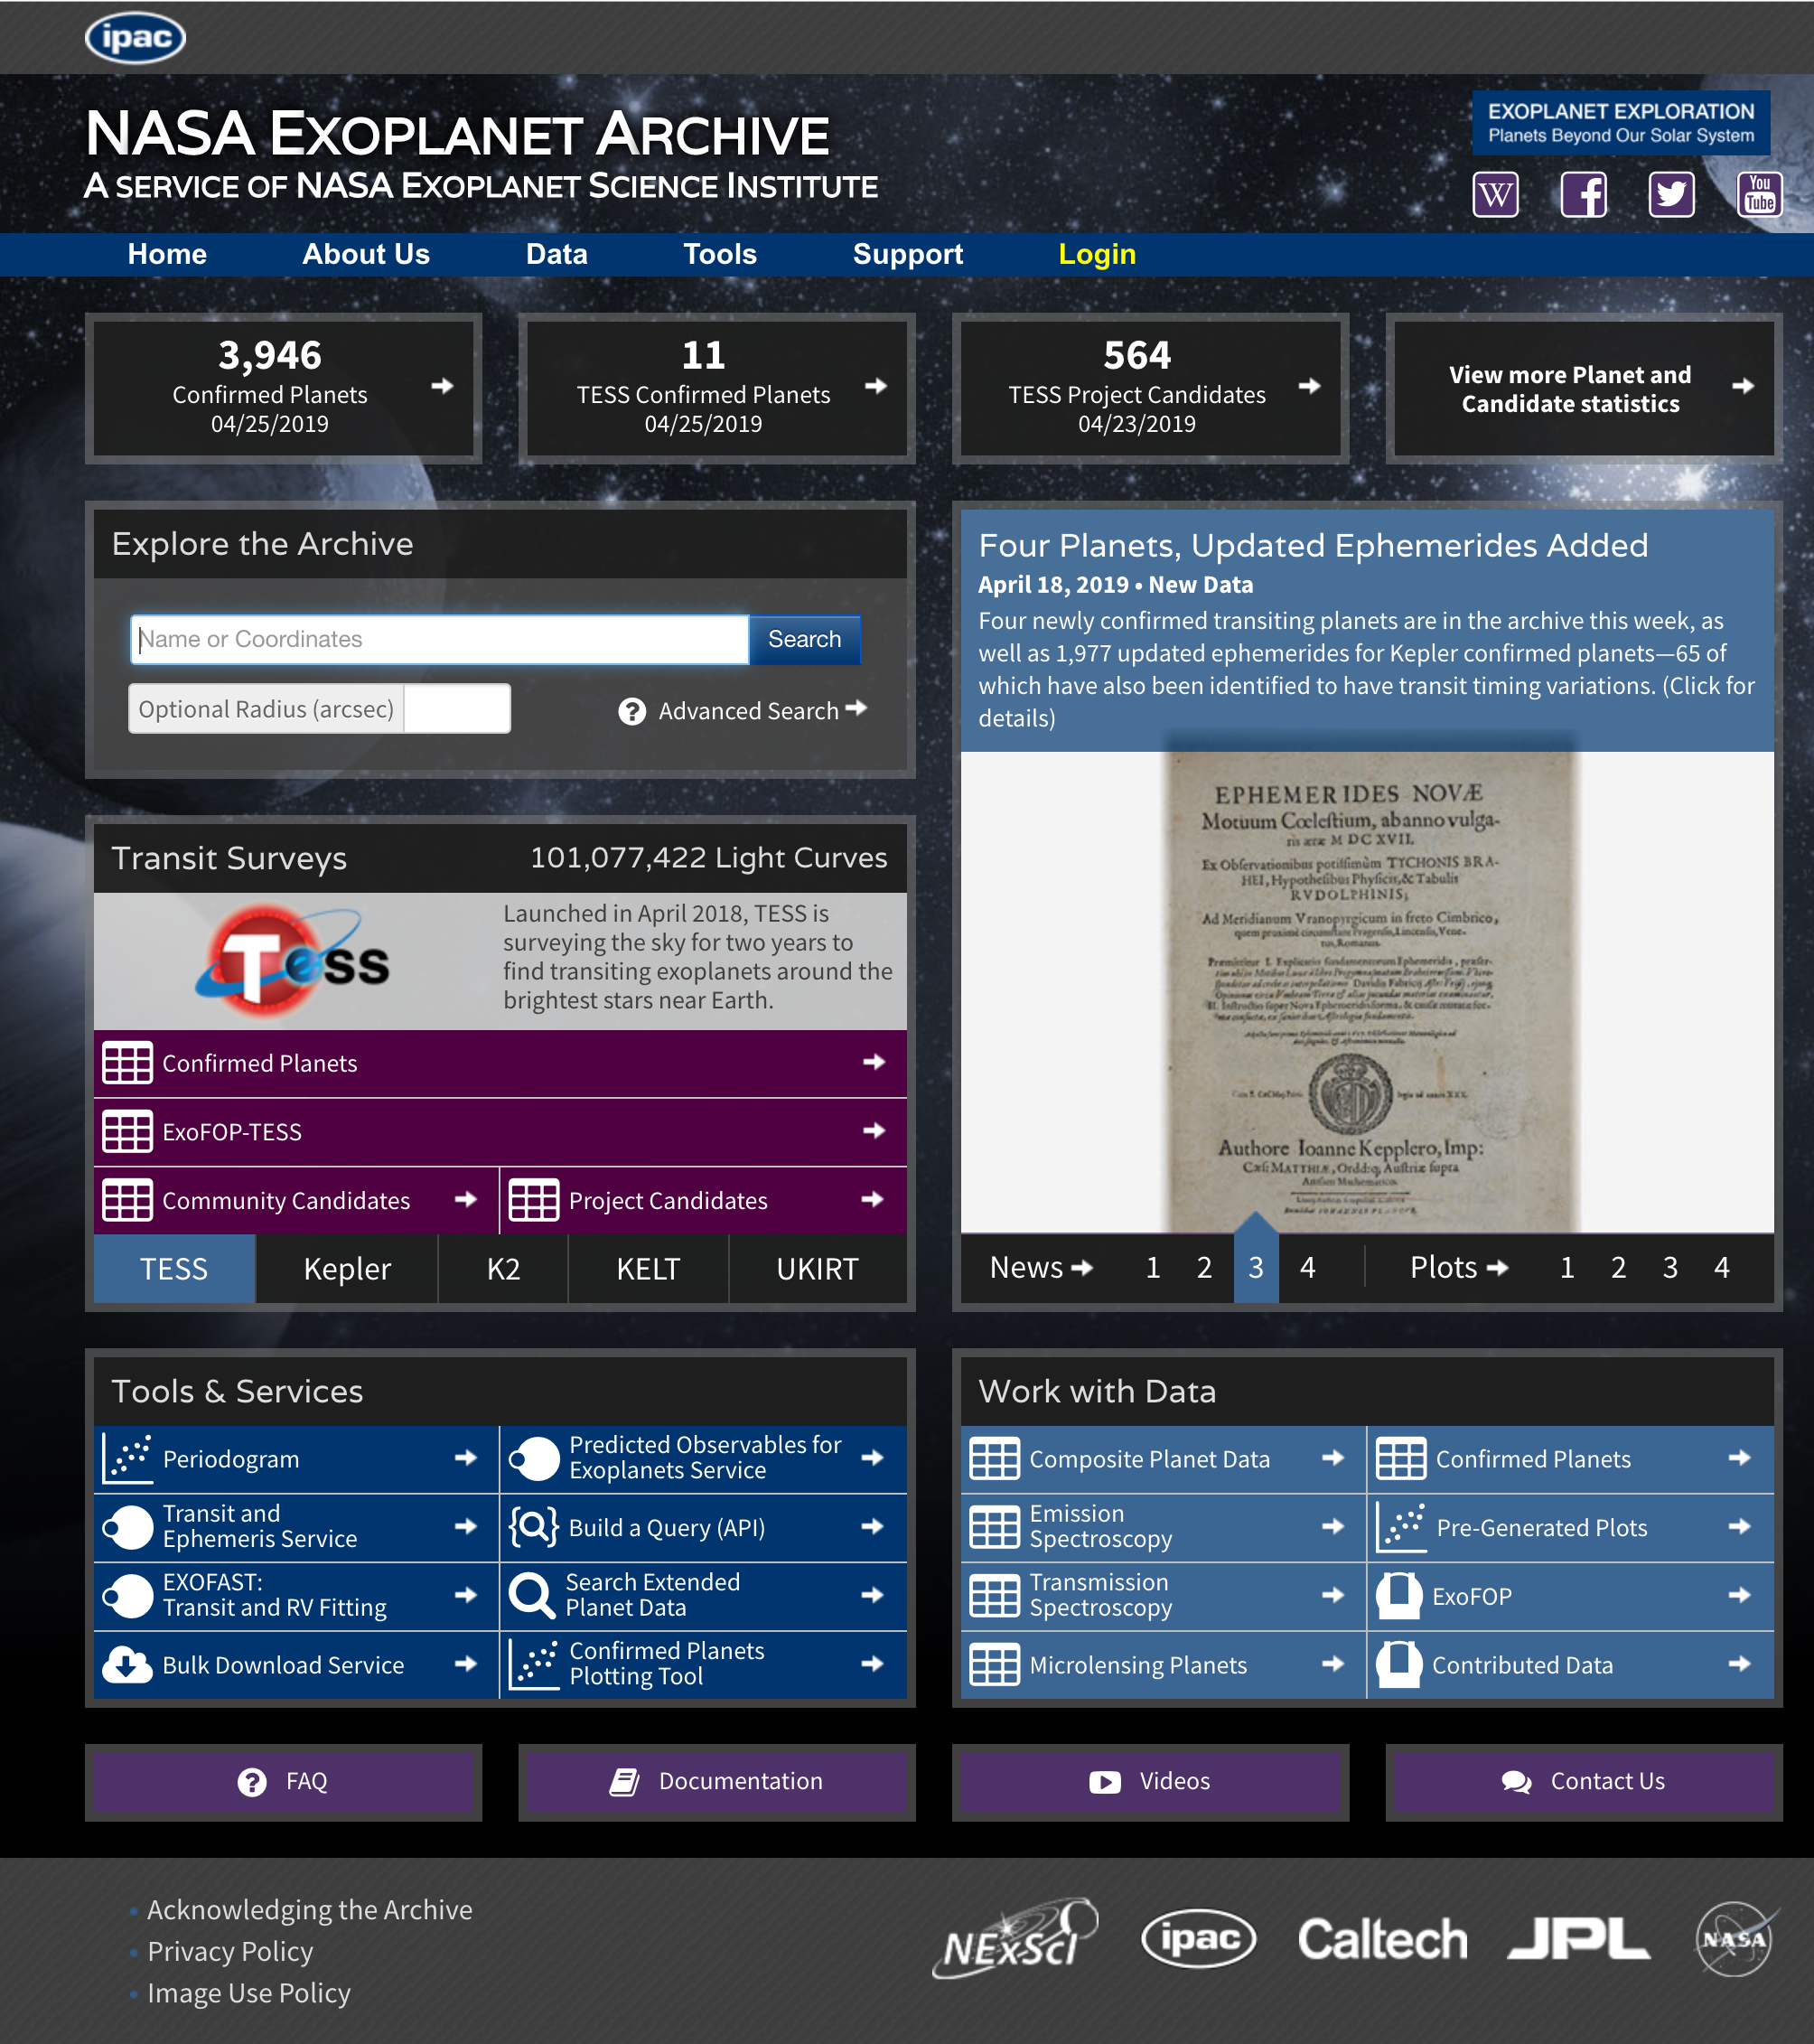
\includegraphics[width=1\linewidth]{screenshot003}
\end{frame}


\begin{frame}
	\frametitle{NASA Publicationsarchiv}
	\begin{figure}
		\centering
		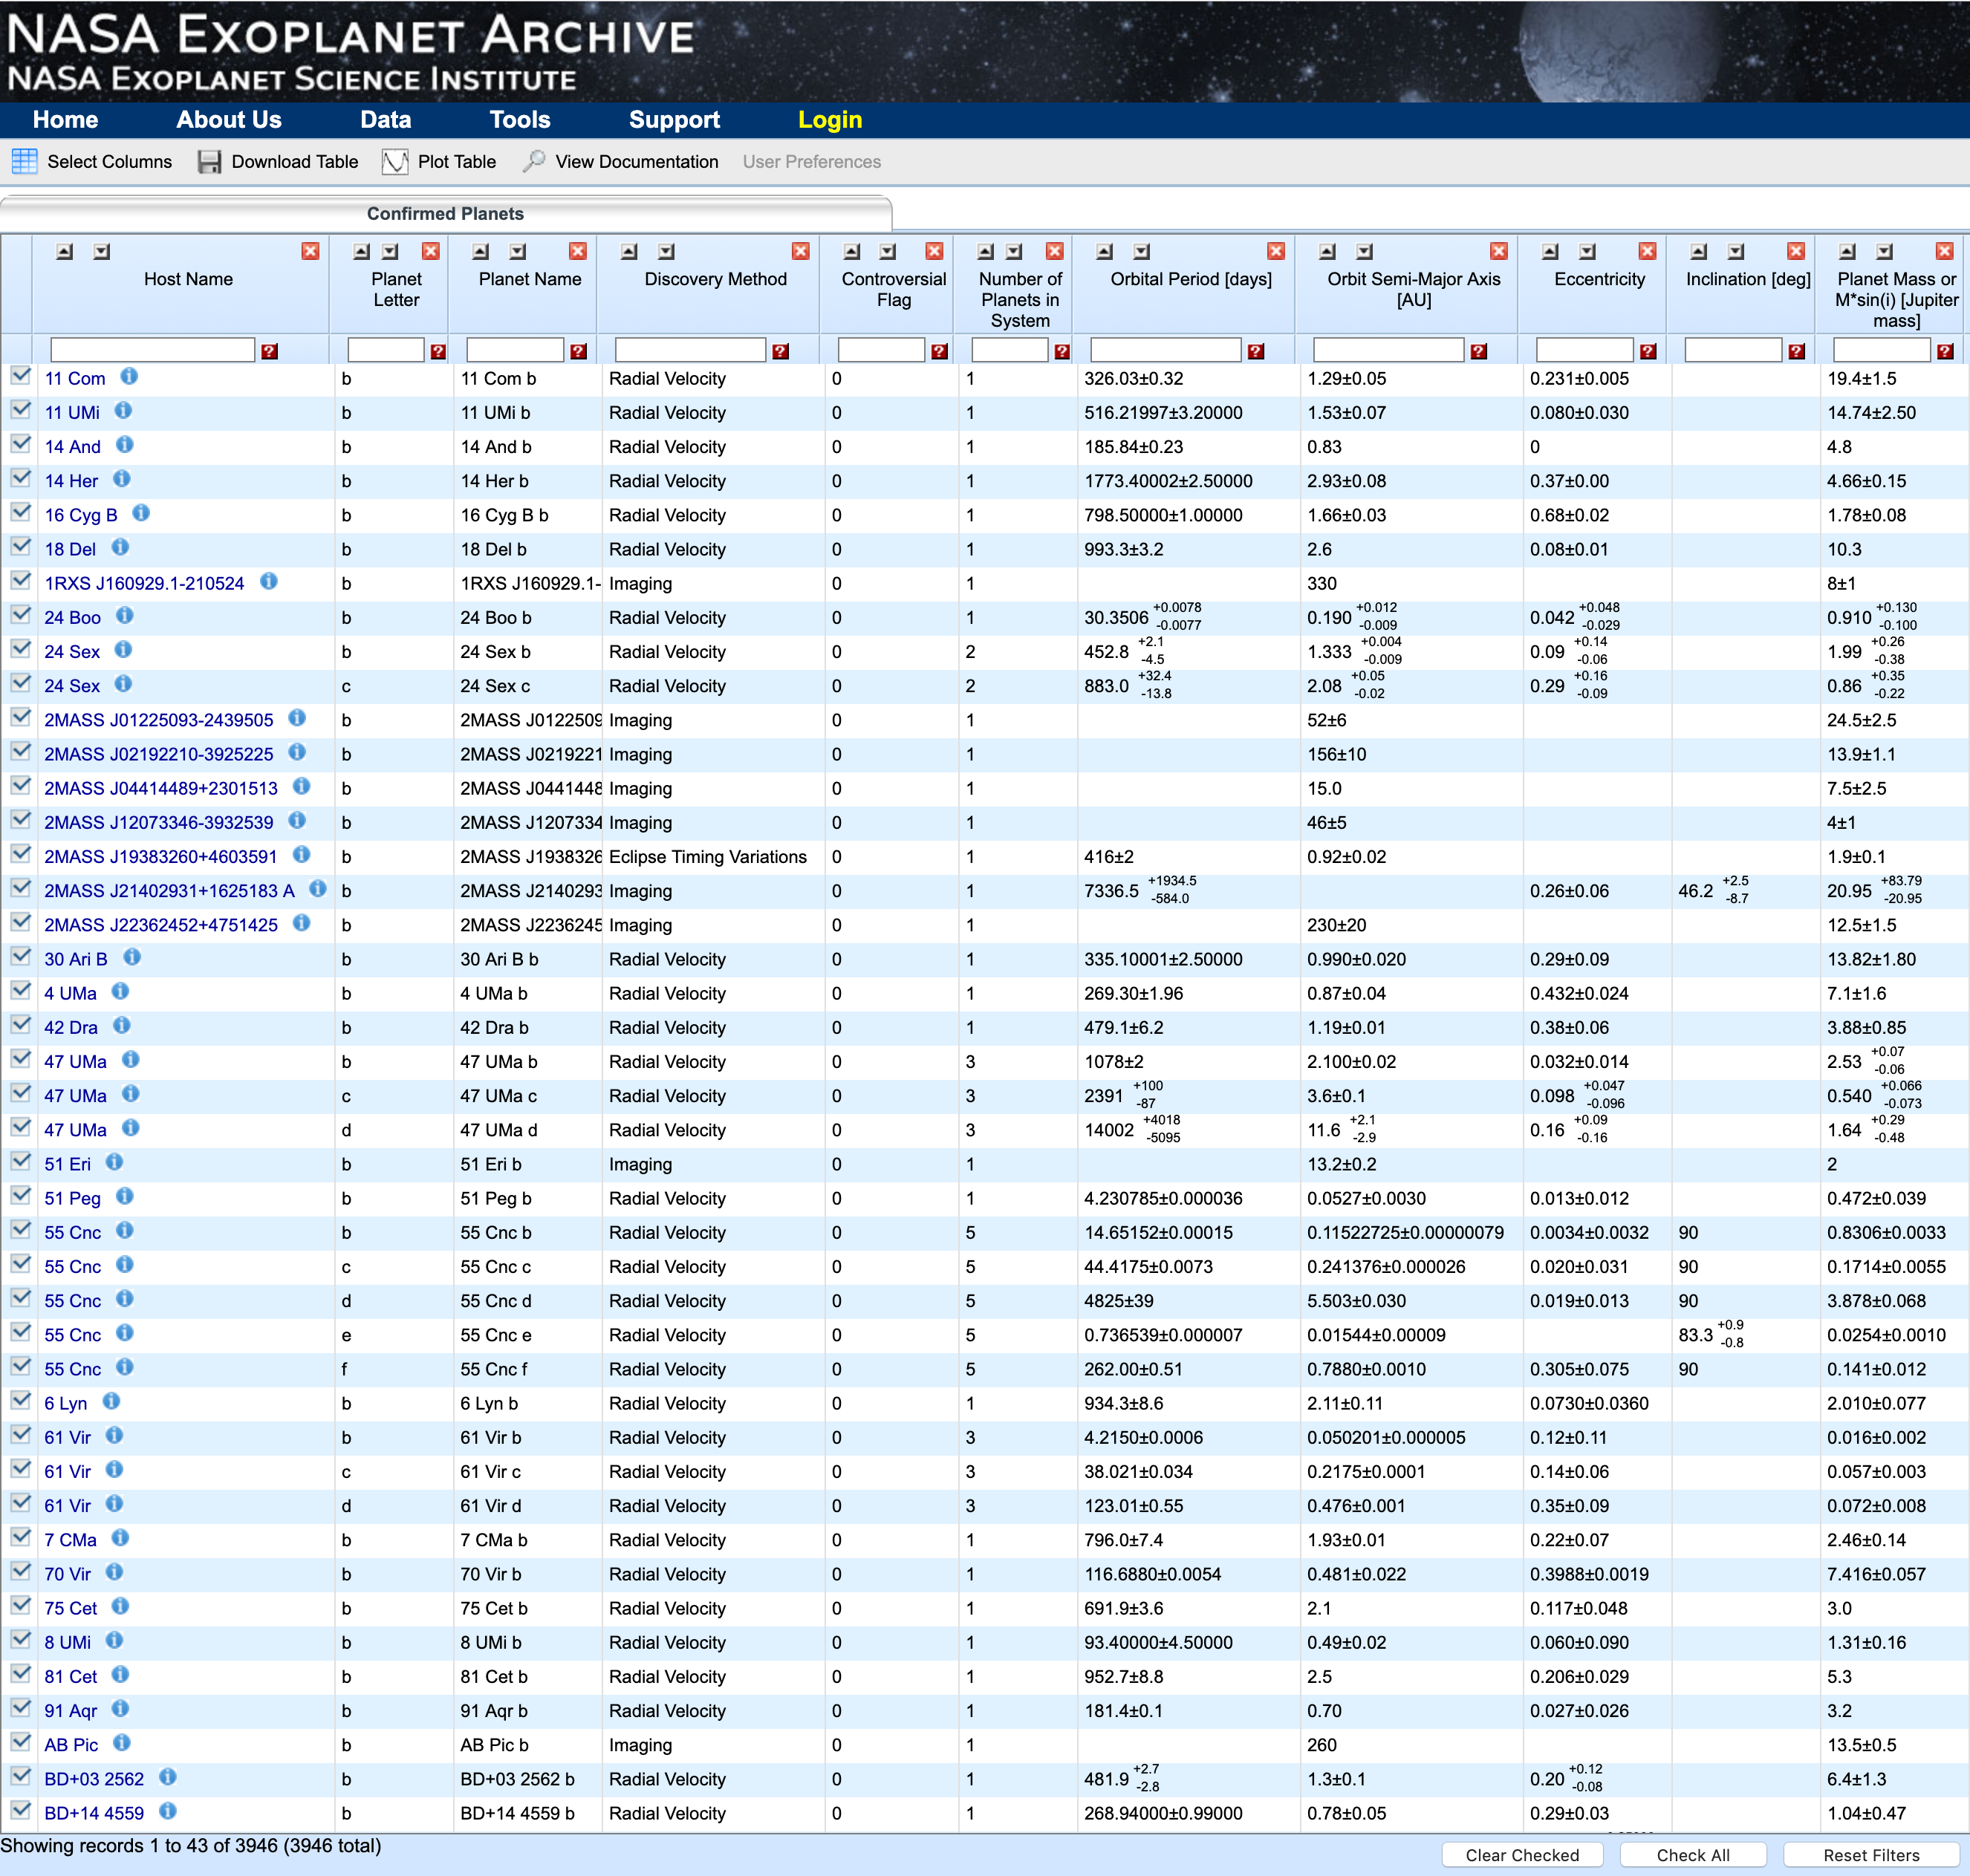
\includegraphics[width=1\linewidth]{screenshot005}
		\caption{}
		\label{fig:screenshot005}
	\end{figure}
\end{frame}

\end{document}